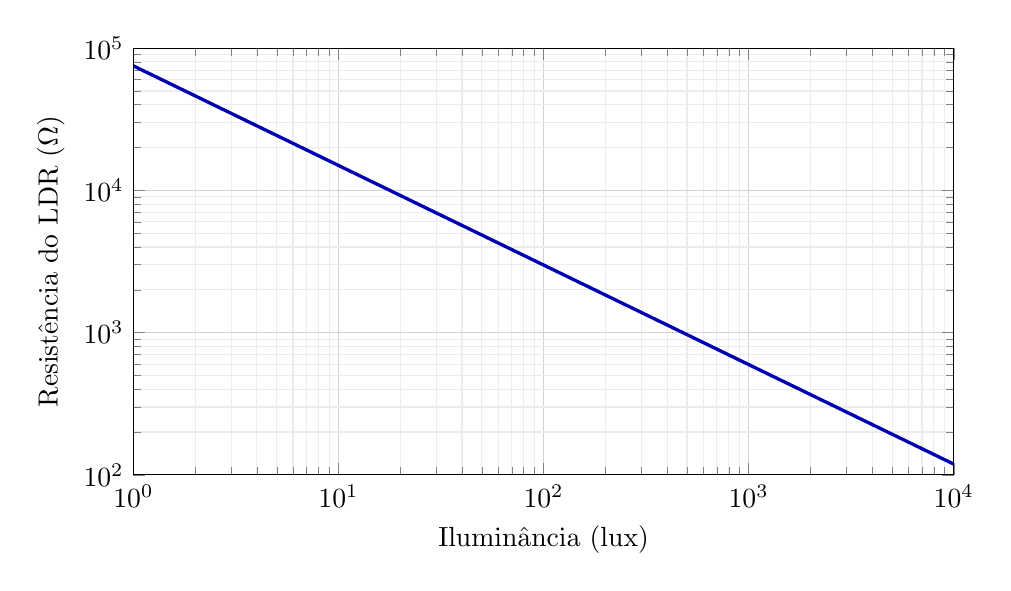
\begin{tikzpicture}
  \begin{loglogaxis}[
    width=12cm, height=7cm,
    xmin=1, xmax=10000, ymin=100, ymax=100000,
    xlabel={Iluminância (lux)},
    ylabel={Resistência do LDR ($\Omega$)},
    grid=both, minor grid style={gray!15}, major grid style={gray!35},
  ]
    \addplot[domain=1:10000, samples=60, very thick, blue!70!black] {75000*x^(-0.7)};
  \end{loglogaxis}
\end{tikzpicture}
